% -*- mode: latex; TeX-engine: xetex; LaTeX-command-style: (("" "SOURCE_DATE_EPOCH=0 %(PDF)%(latex) --shell-escape %S%(PDFout)")); TeX-master: "../dissertation.tex"; -*-

\chapter{Loading of Single Atoms in Optical Tweezer}
\label{ch:loading}

\section{Introduction}
\label{ch:loading:introduction}

The atoms we use in the experiment comes from alkali metal dispensers
heated using an electric current which have a starting temperature of
$\approx\!400\sim800~\mathrm{K}$ and must be cooled to $<\!0.1~\mathrm{K}$
before they can be captured by the optical tweezer.
In this chapter, we will breifly discuss the cooling steps that bridge this temperature gap.
In section \ref{ch:loading:free-space}, we will focus on the free space cooling
on the atoms without involving the optical tweezer.
Since most of the cooling techniques used in our experiment are quite standard,
they will not be reviewed in detail here.
Instead, we will mainly highlight the important specific design choices
and their performance in our experiment as reference.
Section \ref{ch:loading:loading} will discuss the loading and detection
of the atom in the tweezer including a short summary of the unique challenge
we face with Na atoms.
More detail about the apparatus, and the cooling and imaging of the atom
in free space can be found in previous thesis~\cite{liu_building_2019}.

\section{Free Space Cooling of Atoms}
\label{ch:loading:free-space}

\begin{figure}
  \centering
  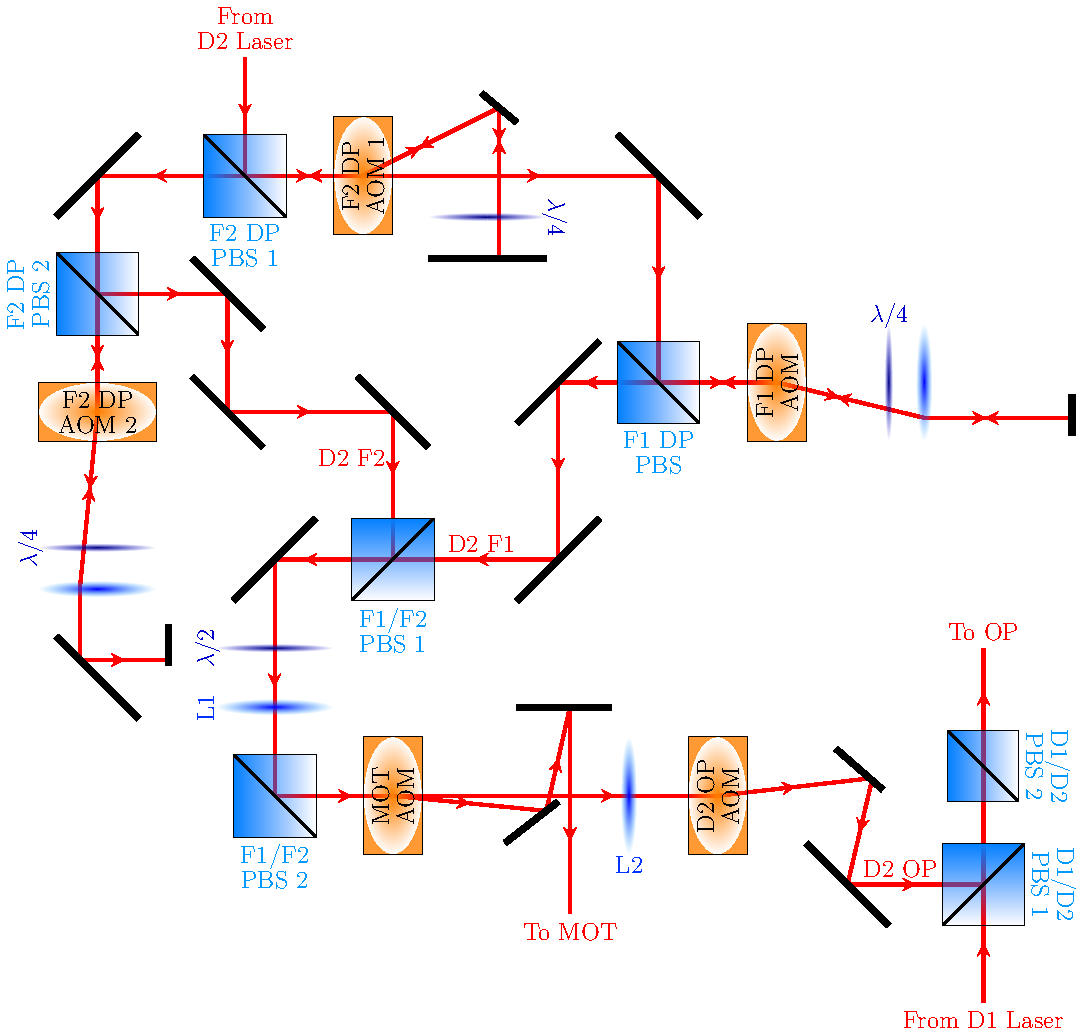
\includegraphics[width=\textwidth]{figures/loading_na_res_beampath.pdf}
  \caption[Beampath for Na $\mathrm{D1}$ and $\mathrm{D2}$ light.]{
    Beampath for generating the frequencies for Na MOT and optical pumping~(OP).
    (Beampath for fiber coupling and frequency locking is not shown.
    The power control for the $\mathrm{D1}$ laser is also omitted.)
    The $\mathrm{D2}$ laser is locked on the $\mathrm{F1}$/$\mathrm{F2}$ crossover line using
    saturated absorption locking.
    It is shifted down by the two $\mathrm{F2}$ double-pass~(DP) AOMs to generate the frequency
    for the Na $F=2$ state and shifted up by the $\mathrm{F1}$ DP AOM
    to address the Na $F=1$ state.
    The frequencies of the $\mathrm{F1}$/$\mathrm{F2}$ light are controlled
    by the $\mathrm{F1}$ DP AOM and $\mathrm{F2}$ DP AOM 2 respectively.
    This set up makes sure that when the $\mathrm{F1}$/$\mathrm{F2}$ DP AOMs are off,
    the closest frequency in the leaked light is at least detuned
    by half the $\mathrm{F1}$/$\mathrm{F2}$
    separation~($\approx\!880~\mathrm{MHz}$)~\cite{steck_sodium_2019}
    and will have minimum effect on the atom.
    The $\mathrm{F1}$ and $\mathrm{F2}$ light are combined
    on $\mathrm{F1}$/$\mathrm{F2}$ PBS 1 and their power ratio after the
    $\mathrm{F1}$/$\mathrm{F2}$ PBS 2 is controlled by the half waveplate between the two PBSs.
    A similar setup is used to combine the $\mathrm{D1}$ and $\mathrm{D2}$ light
    in the OP output using $\mathrm{D1}$/$\mathrm{D2}$ PBS 1
    and the rotating $\mathrm{D1}$/$\mathrm{D2}$ PBS 2.
    Since we need to switch the Na MOT light on and off out-of-phase
    with the Na tweezer~\cite{hutzler_eliminating_2017} at a high frequency,
    the sharpness of the turn on/off edge in the MOT AOM is important.
    We focus the beam through the AOM using lens L1 to optimize the switching time.
    This is then collimated by lens L2 for the downstream beampath.
    \label{fig:loading:free-space:na-res-beampath}}
\end{figure}

\begin{figure}
  \centering
  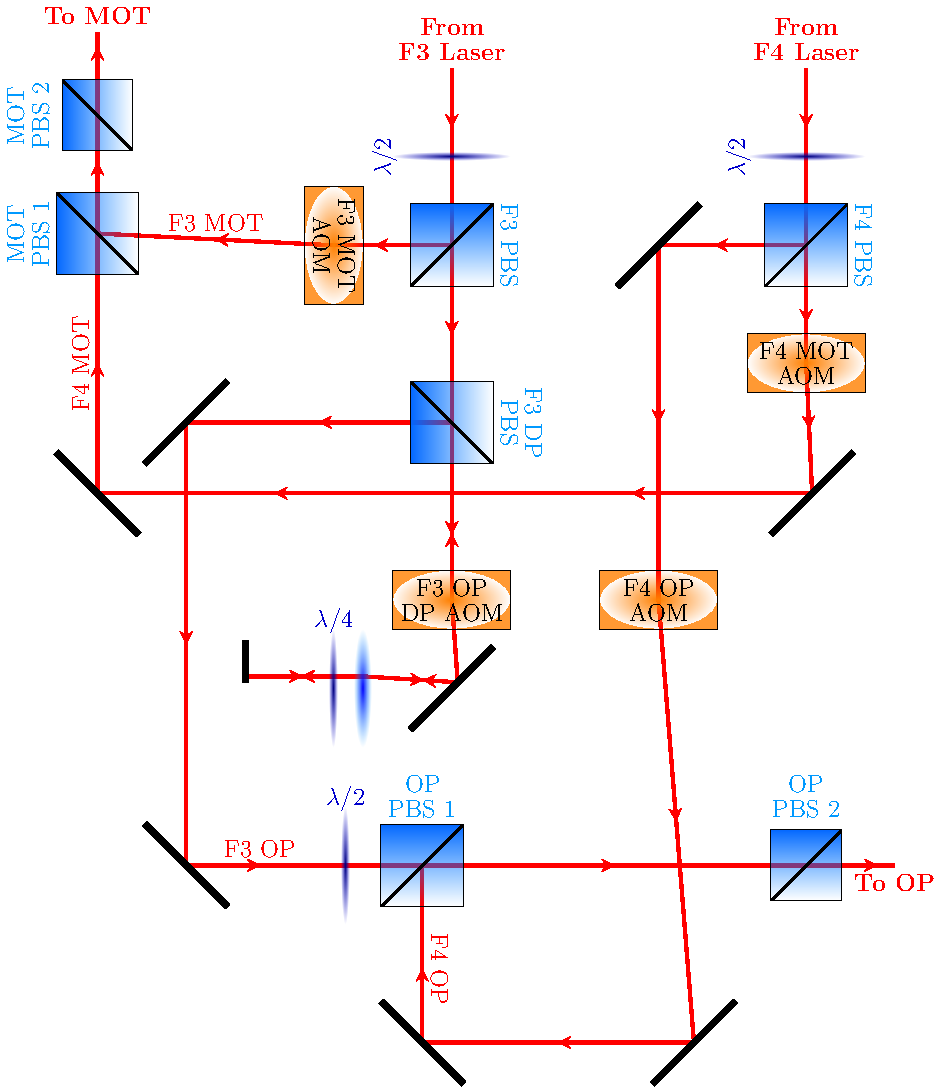
\includegraphics[width=0.866\textwidth]{figures/loading_cs_res_beampath.pdf}
  \caption[Beampath for Cs $\mathrm{D2}$ light.]{
    Beampath for generating the frequencies for Cs MOT and optical pumping~(OP).
    (Beampath for fiber coupling and frequency locking is not shown.)
    The $\mathrm{F3}$ laser is locked using saturated absorption locking
    to the $\mathrm{F3}$ atomic transition.
    The $\mathrm{F4}$ laser is beat-locked to the $\mathrm{F3}$ laser,
    which also controls its frequency.
    The $\mathrm{F3}$ and $\mathrm{F4}$ light are combined on MOT PBS 1 and OP PBS 1
    and their power ratio in the MOT and OP output are controlled by the
    rotating MOT PBS 2 and OP PBS 2 respectively.
    The frequency of the $\mathrm{F3}$ light in the MOT is fixed whereas
    the frequency of the $\mathrm{F3}$ light in the OP
    can be changed by the $\mathrm{F3}$ OP DP AOM.
    \label{fig:loading:free-space:cs-res-beampath}}
\end{figure}

Our experiment begins with the loading of a Na Cs dual species magneto-optical trap~(MOT)
from the background pressure created by the dispensers.
It is created using six cooling beams of $\approx\!4~\mathrm{mm}$ diameter\footnote{
  ISO 11146 diameter~\cite{isotc_172sc_9_iso_2005,dataray_inc_wincamd_2018}}
with $0.5\sim0.9~\mathrm{mW}$~(Na) and $0.3\sim0.5~\mathrm{mW}$~(Cs)
power in each beams.
The resulting MOT has a diameter of $0.1\sim0.2~\mathrm{mm}$
with $10\sim50k$~(Na) and $3\sim20k$~(Cs) atoms being trapped
and cooled to to a temperature of $\approx\!400~\mathrm{mK}$~(Na)
and $\approx\!100~\mathrm{mK}$~(Cs).
The atom numbers are significantly smaller than the ones typically seen in a bulk gas experiment
since the goal of the free-space laser cooling is to load atoms into the tweezers
which does not require large atom numbers.
The small size of the MOT requires a tigher tolerance on the MOT position
in order to overlap with the optical tweezer for the loading of single atoms,
which in turns increased the sensitivity to to the alignment
and power balance of the cooling beams that determines the MOT position.
Because of this, we use four independent fibers to deliver the power
for the four horizontal cooling beams which allows independent control
of the power and alignment.
We observed a more robust MOT and, as a result, single atom loading
compared to using retro-reflectors to create conterpropagating horizontal cooling beams.
Due to the geometric constraints in the experiment,
retro-reflector is used for verticle cooling beams.

The MOT is followed by a compressed-MOT~(CMOT) stage for Na
which uses light closer to resonant to push the Na atoms closer to the center.
After this, the magnetic field is turned off and
a polarization gradient cooling~(PGC) step is applied on the atoms
which cools the atoms to $\approx\!80~\mathrm{mK}$~(Na)
and $\approx\!10~\mathrm{mK}$~(Cs).

The beampaths for generating all the necessary frequencies are shown in
Fig.~\ref{fig:loading:free-space:na-res-beampath}~(Na) and
Fig.~\ref{fig:loading:free-space:cs-res-beampath}~(Cs).
The same beampaths are also used for generating the light for cooling
and imaging of single atoms as well as optical pumping for state preparation
that will be discussed in later chapters.

\section{Loading and Imaging in the Tweezer}
\label{ch:loading:loading}

We load the tweezer from a laser-cooled cloud of atoms.
Since the tweezer provides a conservative potential,
trapping of the atom requires its energy to be reduced.
This can be done either by changing the trap depth,
e.g. turning on the trap when an atom is at the focus to reduce its potential energy,
or by a dissipative cooling process.
However, due to the low trap volume of the tweezer and the density of the MOT,
there is less than $0.01$ atom from the MOT in the tweezer,
and the only method that works for loading tweezer in our experiment
is by cooling the atoms into the tweezer.
This cooling process also ensure that at most one atom can be loaded into the tweezer
due to pair-wise loss from light-assisted collision~\cite{schlosser_sub-poissonian_2001}.

Cooling in tweezer and loading using the free-space cooling beams works well for Cs.
However, the cooling of Na atoms in the tweezer is more challenging
due to the light shift from the tweezer.
The higher trap depth necessary to trap the hotter Na atom after freespace cooling
and the absense of an accessible magic wavelength causes a large ($>\!200~\mathrm{MHz}$)
light shift on the cooling transition when the Na atom is in the tweezer.
This shift significantly changes the cooling detuning making it ineffective in the tweezer.
We fix this issue by alternating the cooling and the tweezer light at $2.5~\mathrm{MHz}$.
The frequency is low enough to allow a few photon to be scattered
when the cooling light is on to perform cooling on the atom,
yet high enough compared to the highest trapping frequency in the tweezer
to prevent parametric heating of the trapped atom~\cite{hutzler_eliminating_2017}.

We use florescence imaging to detect the atoms in the tweezer
which requires cooling to prevent the photon recoil from heating the atom out of the tweezer
before enough photons can be collect.
This is done using the free-space cooling beams previously used for the MOT and the PGC.
The photon scatterred from the atom in the tweezer is collected by the objective
which is then focused onto a EMCCD camera for detection.
We achieve a overall photon collection efficiency of $8~\mathrm{\%}$ and $5~\mathrm{\%}$
for Na and Cs respectively.
The difference between the efficiency for the two atoms
is mainly caused by the quantum efficiency of the camera.

In our experiment, the tweezer is generated by focusing trap light
through an objective with a numerical aperture~(NA) of $0.55$.
The wavelengths used for the tweezers are $700~\mathrm{nm}$ (Na) and $1038~\mathrm{nm}$ (Cs),
which give diffraction limited beam waists of
$0.6~\mathrm{\mu m}$ and $0.9~\mathrm{\mu m}$ respectively.
The selection of the wavelength ensures that each atom can only trapped
by their respective tweezer since,
\begin{enumerate}
\item The Na trap wavelength of $700~\mathrm{nm}$ generates a repulsive potential
  for the Cs atom and therefore cannot trap Cs.
\item The Cs trap can attract Na. However, the Cs trap is not being toggled
  out of phase with the Na cooling light and therefore cannot trap Na due to the light shift.
\end{enumerate}
Due to technical limitations, we cannot measure the tweezer power directly.
Instead we measure the power upstream in the tweezer beampath where the beam is accessible
and correct for the known total transmission efficiency of $23(2)~\mathrm{\%}$ from the optics.
The tweezer powers quoted in this thesis are directly measured power
and must be multiplied by the factor $0.23$ to obtain
the best estimate of the total power at the focus of the tweezer.

\begin{figure}
  \centering
  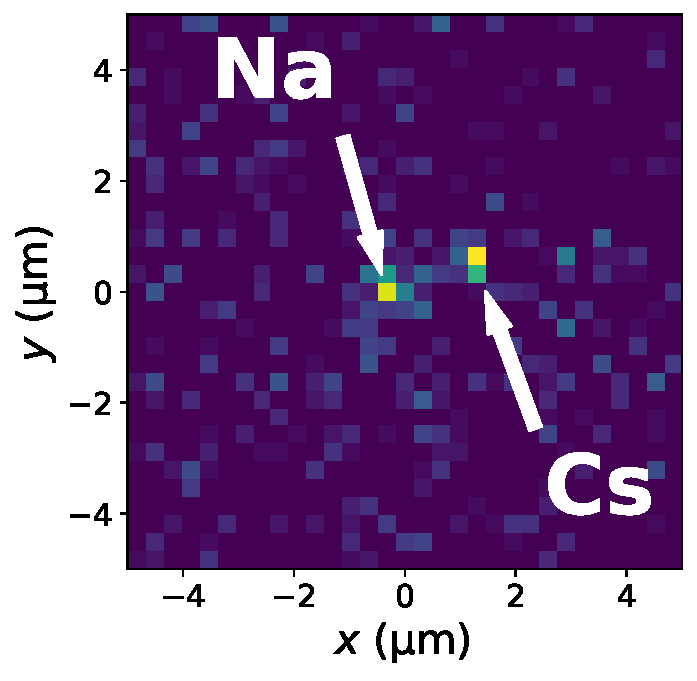
\includegraphics[width=0.5\textwidth]{figures/loading_single_atoms.pdf}
  \caption[Image of single Na and Cs atoms.]{
    Image of a single Na and Cs atoms in their respective tweezers
    showing a simultaneous loading event.
    \label{fig:loading:loading:single-atoms}}
\end{figure}

The single atom can be observed on the EMCCD camera if the tweezer beam
is turned on during MOT loading and the loading efficiency is improved
by the additional free-space cooling steps including CMOT and PGC.
Fig.~\ref{fig:loading:loading:single-atoms} shows a image of both the Na and Cs atoms.
In most experiments, however, the two species are imaged separately
in order to reduce the background and to improve the detection fidelity.
We take a image for each atoms right after the loading step in order to determine
which atoms (if any) are loaded and this is repeated at the end of each experimental sequences
to determine if the atoms have survived.
By repeating the experiment and sorting the events according to the loading result,
we can accurately identify the case where a single (Na or Cs) or a pair of atoms are loaded
and estimate the corresponding single- and two-body survival probability.
Most of the measurements in this thesis are based on this probability.

\section{Summary and Outlook}
\label{ch:loading:summary}

In this chapter we discussed the trapping and imaging of the single atoms in the optical
tweezers and the steps leading up to it.
We take advantage of many techniques developped and used in previous experiments
to boost our control on the atoms in preparation for the control on the molecules.

The atoms trapped in the tweezers and the high fidelity detection of them
form the fundation of our experiment.
The utility of such system and the possibility it opens up will be discussed
in more detail in the coming chapters.
